\documentclass[11pt,oneside]{article}	%use"amsart"insteadof"article"forAMSLaTeXformat
\usepackage{geometry}		%Seegeometry.pdftolearnthelayoutoptions.Therearelots.
\geometry{letterpaper}		%...ora4paperora5paperor...
%\geometry{landscape}		%Activateforforrotatedpagegeometry
%\usepackage[parfill]{parskip}		%Activatetobeginparagraphswithanemptylineratherthananindent
\usepackage{graphicx}				%Usepdf,png,jpg,orepsßwithpdflatex;useepsinDVImode
								%TeXwillautomaticallyconverteps-->pdfinpdflatex		
\usepackage{amssymb}
\usepackage[colorlinks]{hyperref}

%----macros begin---------------------------------------------------------------
\usepackage{color}
\usepackage{amsthm}

\def\conv{\mbox{\textrm{conv}\,}}
\def\aff{\mbox{\textrm{aff}\,}}
\def\E{\mathbb{E}}
\def\R{\mathbb{R}}
\def\Z{\mathbb{Z}}
\def\tex{\TeX}
\def\latex{\LaTeX}
\def\v#1{{\bf #1}}
\def\p#1{{\bf #1}}
\def\T#1{{\bf #1}}

\def\vet#1{{\left(\begin{array}{cccccccccccccccccccc}#1\end{array}\right)}}
\def\mat#1{{\left(\begin{array}{cccccccccccccccccccc}#1\end{array}\right)}}

\def\lin{\mbox{\rm lin}\,}
\def\aff{\mbox{\rm aff}\,}
\def\pos{\mbox{\rm pos}\,}
\def\cone{\mbox{\rm cone}\,}
\def\conv{\mbox{\rm conv}\,}
\newcommand{\homog}[0]{\mbox{\rm homog}\,}
\newcommand{\relint}[0]{\mbox{\rm relint}\,}

%----macros end-----------------------------------------------------------------

\title{Boolean combination of cellular complexes
\footnote{This document is part of the \emph{Linear Algebraic Representation with CoChains} (LAR-CC) framework~\cite{cclar-proj:2013:00}. \today}
}
\author{Alberto Paoluzzi}
%\date{}							%Activatetodisplayagivendateornodate

\begin{document}
\maketitle
\tableofcontents
\nonstopmode

\section{Introduction}

\section{Merging arguments}

\paragraph{Building a covering of common convex hull}

%-------------------------------------------------------------------------------
@D Building a covering of common convex hull
@{def covering(model1,model2):
	V, CV1, CV2, n12 = vertexSieve(model1,model2)
	_,EEV1 = larFacets((V,CV1),dim=2,emptyCellNumber=1)
	_,EEV2 = larFacets((V,CV2),dim=2,emptyCellNumber=1)
	CV1 = CV1[:-1]
	CV2 = CV2[:-1]
	VV = AA(LIST)(range(len(V)))
	return V,[VV,EEV1,EEV2,CV1,CV2],n12
@}
%-------------------------------------------------------------------------------

\begin{figure}[htbp] %  figure placement: here, top, bottom, or page
   \centering
   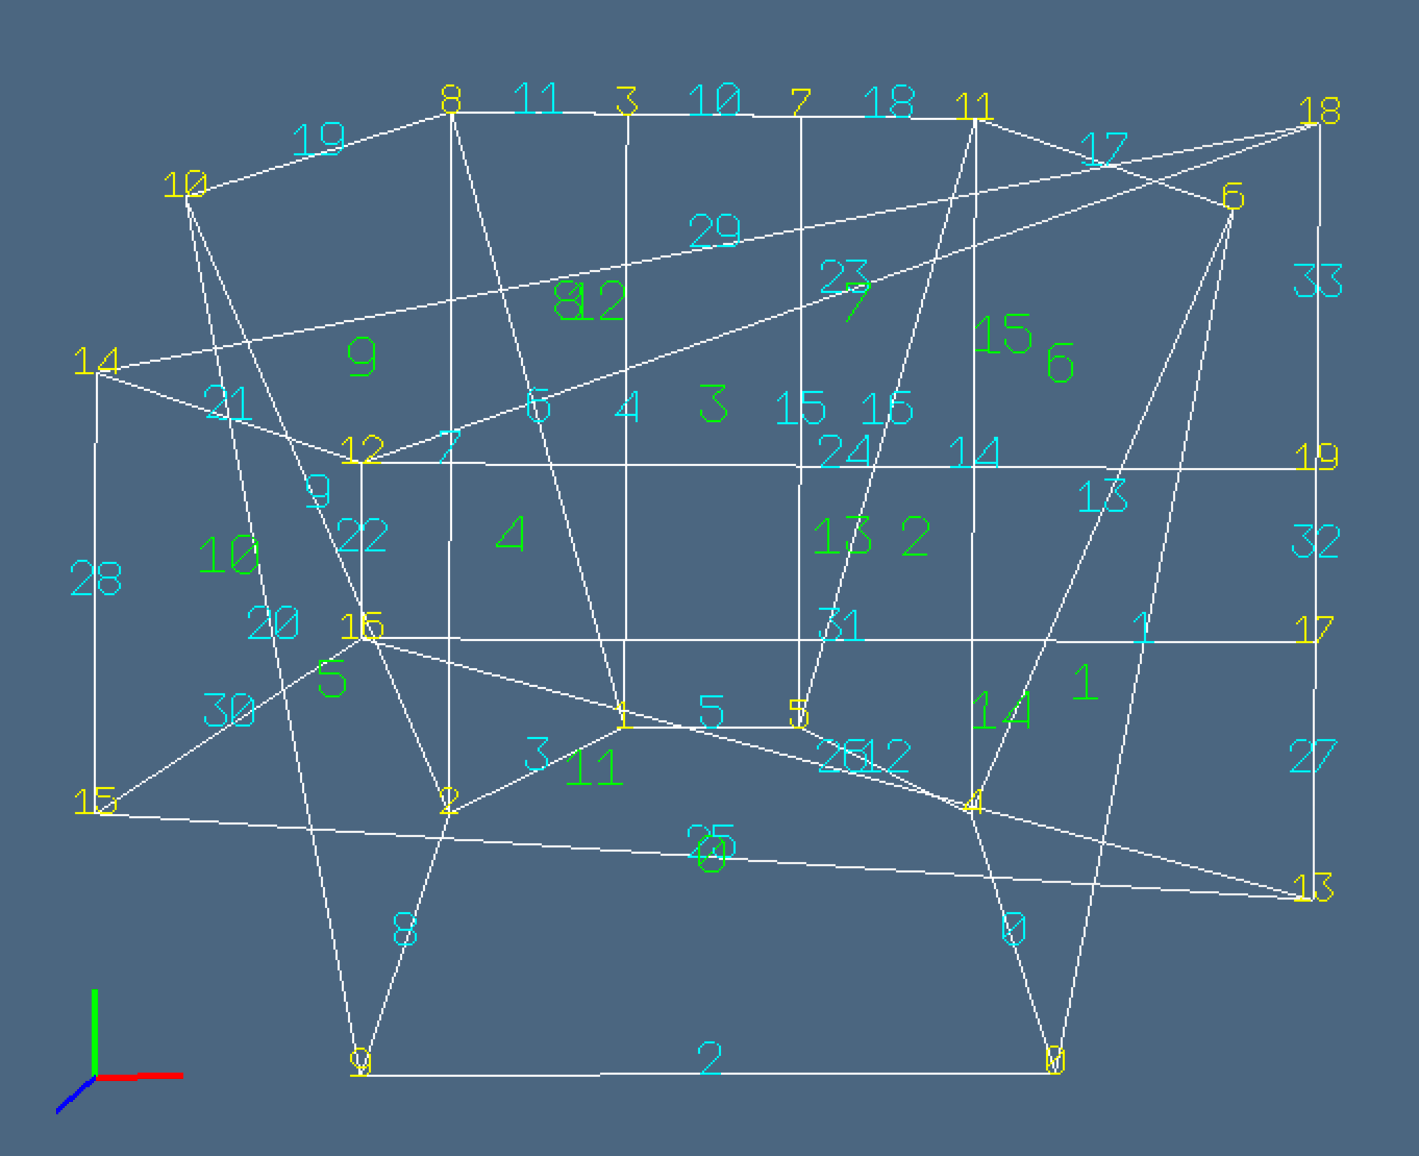
\includegraphics[width=0.6\linewidth]{images/covering} 
   \caption{Set covering of the two Boolean arguments.}
   \label{fig:example}
\end{figure}

\paragraph{Building a partition of common convex hull}

%-------------------------------------------------------------------------------
@D Building a partition of common convex hull of vertices
@{def partition(V, CV1,CV2, EEV1,EEV2):
	CV = sorted(AA(sorted)(Delaunay(array(V)).vertices))
	BV1, BV2, BF1, BF2 = boundaryVertices( V, CV1,CV2, 'cuboid', EEV1,EEV2 )
	BV = BV1+BV2
	nE1 = len(EEV1)
	BF = BF1+[e+nE1 for e in BF2]
	return CV, BV1, BV2, BF1, BF2, BV, BF, nE1
@}
%-------------------------------------------------------------------------------




\section{Selecting cells to split}


\paragraph{Relational inversion (Characteristic matrix transposition)}

%-------------------------------------------------------------------------------
@D Characteristic matrix transposition
@{""" Characteristic matrix transposition """
def invertRelation(V,CV):
	VC = [[] for k in range(len(V))]
	for k,cell in enumerate(CV):
		for v in cell:
			VC[v] += [k]
	return VC
@}
%-------------------------------------------------------------------------------


%-------------------------------------------------------------------------------
@D Look for cells in Delaunay, with vertices in both operands
@{""" Look for cells in Delaunay, with vertices in both operands """
def mixedCells(CV,n0,n1,m0,m1):
	return [list(cell) for cell in CV if any([ n0<=v<=n1 for v in cell]) 
		and any([ m0<=v<=m1 for v in cell])]
@}
%-------------------------------------------------------------------------------

%-------------------------------------------------------------------------------
@D Look for cells in cells12, with vertices on boundaries
@{""" Look for cells in cells12, with vertices on boundaries """
def mixedCellsOnBoundaries(cells12,BV1,BV2):
	cells12BV1 = [cell for cell in cells12
					if len(list(set(cell).intersection(BV1))) != 0]
	cells12BV2 = [cell for cell in cells12
					if len(list(set(cell).intersection(BV2))) != 0]
	pivots = sorted(AA(sorted)(cells12BV1+cells12BV2))
	pivots = [cell for k,cell in enumerate(pivots[:-1]) if cell==pivots[k+1]]
	return pivots
@}
%-------------------------------------------------------------------------------

%-------------------------------------------------------------------------------
@D Build intersection tasks
@{""" Build intersection tasks """
def cuttingTest(cuttingHyperplane,polytope,V):
	signs = [INNERPROD([cuttingHyperplane, V[v]+[1.]]) for v in polytope]
	return any([value<0 for value in signs]) and any([value>0 for value in signs])

def splittingTasks(V,pivots,BV,BF,VC,CV,EEV,VE):
	tasks = []
	for pivotCell in pivots:
		cutVerts = [v for v in pivotCell if v in BV]
		for v in cutVerts:
			cutFacets = [e for e in VE[v] if e in BF]
			cells2cut = VC[v]
			for facet,cell2cut in CART([cutFacets,cells2cut]):
				polytope = CV[cell2cut]
				points = [V[w] for w in EEV[facet]]
				dim = len(points[0])
				theMat = Matrix( [(dim+1)*[1.]] + [p+[1.] for p in points] )
				cuttingHyperplane = [(-1)**(col)*theMat.minor(0,col).determinant() 
									for col in range(dim+1)]
				if cuttingTest(cuttingHyperplane,polytope,V):
					tasks += [[facet,cell2cut,cuttingHyperplane]]
	tasks = AA(eval)(set(AA(str)(tasks)))
	tasks = TrivialIntersection(tasks,V,EEV,CV)
	print "\ntasks =",tasks
	return tasks
@}
%-------------------------------------------------------------------------------

\paragraph{facet-cell trivial intersection filtering}

A final filtering is applied to the pairs \texttt{(cuttingHyperplane,polytope} in the \texttt{tasks} array, in order to remove those pairs whose intersection reduces to a single point, i.e.~to the comman vertex between the boundary $(d-1)$-face, having \texttt{cuttingHyperplane} as affine hull, and the \texttt{polytope} $d$-cell.

For this purpose, it is checked that at leaf one of the facet vertices, transformed into the common-vertex-based coordinate frame, have all positive coordinates. This fact guarantees the existence of a non trivial intersection between the $(d-1)$-face and the $d$-cell.

%-------------------------------------------------------------------------------
@D Trivial intersection filtering
@{""" Trivial intersection filtering """
def TrivialIntersection(tasks,V,EEV,CV):
	out = []
	for face,cell,affineHull in tasks:
		faceVerts, cellVerts = EEV[face], CV[cell]
		v0 = list(set(faceVerts).intersection(cellVerts))[0] # v0 = common vertex
		transformMat = mat([VECTDIFF([V[v],V[v0]]) for v in cellVerts if v != v0]).I
		vects = (transformMat * mat([VECTDIFF([V[v],V[v0]]) for v in faceVerts 
					if v != v0]).T).tolist()
		if any([all([x>0 for x in list(vect)]) for vect in vects]): out += [[face,cell,affineHull]]
	return out
@}
%-------------------------------------------------------------------------------


\section{Splitting cells traversing the boundaries}

In the previous section we computed a set of "slitting seeds", each made by a boundary facet and by a Delaunay cell to be splitted by the facet's affine hull. Here we show how to partition ate each such cells into two cells, according to Figure~\ref{fig:splitting}, where the boundary facets of the two boolean arguments are shown in yellow color.

\begin{figure}[htbp] %  figure placement: here, top, bottom, or page
   \centering
   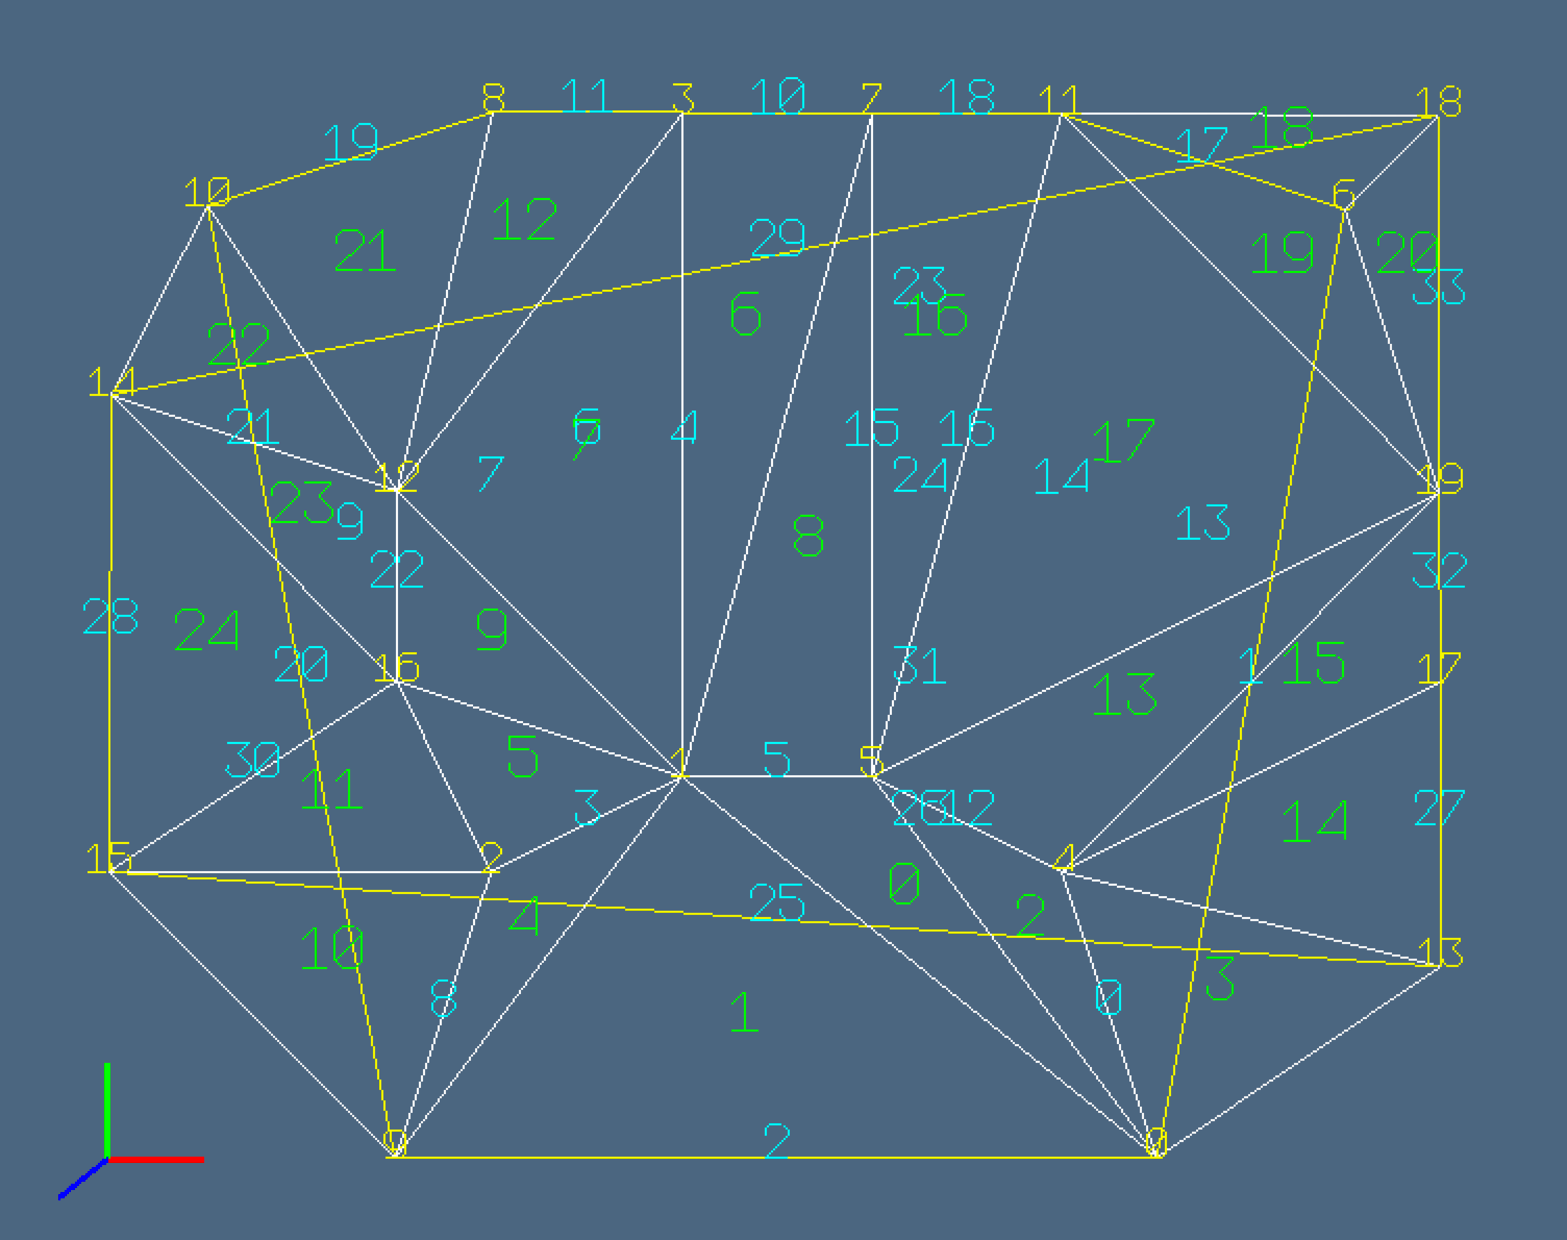
\includegraphics[width=0.6\linewidth]{images/splitting} 
   \caption{example caption}
   \label{fig:splitting}
\end{figure}

In the example in Figure~\ref{fig:splitting}, the set of pairs \texttt{(facet,cell)} to be used as splitting seeds are given below.
{\small
\begin{verbatim}
[[25, 3], [1, 3], [29, 18], [20, 22], [1, 19], [25, 10], [20, 10], [29, 22]]
\end{verbatim}}

\subsection{Cell splitting}

A cell will be split by pyplasm intersection with a suitable rotated and translated instance of a (large) $d$-cuboid with the superior face embedded in the hyperplane $z=0$.

\paragraph{Splitting a cell with an hyperplane}
The macro below defines a function \texttt{cellSplitting}, with input the index of the \texttt{face}, the index of the \texttt{cell} to be bisected, the \texttt{covector} giving the coefficients of the splitting hyperplane, i.e.~the affine hull of the splitting \texttt{face}, and the arrays \texttt{V}, \texttt{EEV}, \texttt{CV}, giving the coordinates of vertices, the (accumulated) facet to vertices relation (on the input models), and the cell to vertices relation (on the Delaunay model), respectively. 

The actual subdivision of the input \texttt{cell} onto the two output cells \texttt{cell1} and \texttt{cell2} is performed by using the \texttt{pyplasm} Boolean operations of intersection and difference of the input with a solid simulation of the needed hyperspace, provided by the \texttt{rototranslSubspace} variable. Of course, such pyplasm operators return two Hpc values, whose vertices will then extracted using the \texttt{UKPOL} primitive.

%-------------------------------------------------------------------------------
@D Cell splitting
@{""" Cell splitting in two cells """
def cellSplitting(face,cell,covector,V,EEV,CV):
	dim = len(V[0])
	subspace = (T(range(1,dim+1))(dim*[-50])(CUBOID(dim*[100])))
	normal = covector[:-1]
	if len(normal) == 2:  # 2D complex
		rotatedSubspace = R([1,2])(ATAN2(normal)-PI/2)(T(2)(-50)(subspace))
	elif len(normal) == 3:  # 3D complex
		rotatedSubspace = R()()(subspace)
	else: print "rotation error"
	t = V[EEV[face][0]]
	rototranslSubspace = T(range(1,dim+1))(t)(rotatedSubspace)
	cellHpc = MKPOL([V,[[v+1 for v in CV[cell]]],None])
	print "\ncell =",UKPOL(cellHpc)[0]
	# cell1 = INTERSECTION([cellHpc,rototranslSubspace])
	
	tolerance=0.0001
	use_octree=False
	cell1 = Plasm.boolop(BOOL_CODE_AND, 
		[cellHpc,rototranslSubspace],tolerance,plasm_config.maxnumtry(),use_octree)
	
	# cell2 = DIFFERENCE([cellHpc,rototranslSubspace])
	
	cell2 = Plasm.boolop(BOOL_CODE_DIFF, 
		[cellHpc,rototranslSubspace],tolerance,plasm_config.maxnumtry(),use_octree)

	return cell1,cell2
@}
%-------------------------------------------------------------------------------


\section{Reconstruction of results}

\section{Exporting the library}


%-------------------------------------------------------------------------------
@O lib/py/bool.py
@{""" Module for Boolean ops with LAR """
from matrix import *
@< Initial import of modules @>
@< Symbolic utility to represent points as strings @>
@< Building a covering of common convex hull @>
@< Building a partition of common convex hull of vertices @>
@< Characteristic matrix transposition @>
@< Look for cells in Delaunay, with vertices in both operands @>
@< Look for cells in cells12, with vertices on boundaries @>
@< Build intersection tasks @>
@< Trivial intersection filtering @>
@< Cell splitting @>
@}
%-------------------------------------------------------------------------------

\section{Tests}

\subsection{2D examples}

\subsubsection{First examples}


Three sets of input 2D data are prepared here, ranging from very simple to a small instance of the hardest kind of dataset, known to produce an output of size $O(n^2)$.


%-------------------------------------------------------------------------------
@D First set of 2D data: Fork-0 input
@{""" Definition of Boolean arguments """
V1 = [[3,0],[11,0], [13,10], [10,11], [8,11], [6,11], [4,11], [1,10], [4,3], [6,4], 
	[8,4], [10,3]]
FV1 = [[0,1,8,9,10,11],[1,2,11], [3,10,11], [4,5,9,10], [6,8,9], [0,7,8], [2,3,11],
	[3,4,10], [5,6,9], [6,7,8], range(8)]
V2 = [[0,3],[14,2], [14,5], [14,7], [14,11], [0,8], [3,7], [3,5]]
FV2 =[[0,5,6,7], [0,1,7], [4,5,6], [2,3,6,7], [1,2,7], [3,4,6], range(6)]
@}
%-------------------------------------------------------------------------------


\paragraph{Input and visualisation of Boolean arguments}

%-------------------------------------------------------------------------------
@D Computation of lower-dimensional cells
@{""" Computation of edges an input visualisation """
model1 = V1,FV1
model2 = V2,FV2
submodel = SKEL_1(STRUCT(MKPOLS(model1)+MKPOLS(model2)))
VV1 = AA(LIST)(range(len(V1)))
_,EV1 = larFacets((V1,FV1),dim=2,emptyCellNumber=1)
VV2 = AA(LIST)(range(len(V2)))
_,EV2 = larFacets((V2,FV2),dim=2,emptyCellNumber=1)
VIEW(larModelNumbering(V1,[VV1,EV1,FV1],submodel,4))
VIEW(larModelNumbering(V2,[VV2,EV2,FV2],submodel,4))
@}
%-------------------------------------------------------------------------------

\paragraph{Exporting test file}

%-------------------------------------------------------------------------------
@D Bulk of Boolean task computation
@{""" Bulk of Boolean task computation """
@< Computation of lower-dimensional cells @>
V,[VV,EEV1,EEV2,CV1,CV2],n12 = covering(model1,model2)
CCV = CV1+CV2
EEV = EEV1+EEV2
VIEW(larModelNumbering(V,[VV,EEV,CCV],submodel,4))

CV, BV1, BV2, BF1, BF2, BV, BF, nE1 = partition(V, CV1,CV2, EEV1,EEV2)
boundaries = COLOR(YELLOW)(SKEL_1(STRUCT(MKPOLS((V,[EEV[e] for e in BF])))))
submodel = STRUCT([ SKEL_1(STRUCT(MKPOLS((V,CV)))), boundaries ])
VIEW(larModelNumbering(V,[VV,EEV,CV],submodel,4))
@< Inversion of incidences @>

n0,n1 = 0, max(AA(max)(CV1))			# vertices in CV1 (extremes included)
m0,m1 = n1+1-n12, max(AA(max)(CV2))		# vertices in CV2 (extremes included)
VE = [VEE1[v]+VEE2[v] for v in range(len(V))]
cells12 = mixedCells(CV,n0,n1,m0,m1)
pivots = mixedCellsOnBoundaries(cells12,BV1,BV2)
tasks = splittingTasks(V,pivots,BV,BF,VC,CV,EEV,VE)
print "\ntasks (facet,cell2cut) =",tasks

out = []
for task in tasks:
	face,cell,covector = task
	cell1,cell2 = cellSplitting(face,cell,covector,V,EEV,CV)
	verts,cells,pols = UKPOL(cell1)
	print "\n cell1 =",AA(vcode)(verts), cells, pols
	verts,cells,pols = UKPOL(cell2)
	print " cell2 =",AA(vcode)(verts), cells, pols
	out += [ COLOR(GREEN)(cell2), COLOR(CYAN)(cell1) ]
	
VIEW(STRUCT([ STRUCT(out), submodel ]))
@}
%-------------------------------------------------------------------------------


%-------------------------------------------------------------------------------
@O test/py/bool/test01.py
@{
import sys
""" import modules from larcc/lib """
sys.path.insert(0, 'lib/py/')
from bool import *
@< First set of 2D data: Fork-0 input @>
@< Bulk of Boolean task computation @>
@}
%-------------------------------------------------------------------------------


\paragraph{association of cells and boundaries}

%-------------------------------------------------------------------------------
@D Inversion of incidences
@{""" Inversion of incidences """
VC = invertRelation(V,CV)
VC1 = invertRelation(V,CV1)
VC2 = invertRelation(V,CV2)
VEE1 = invertRelation(V,EEV1)
VEE2 = [[e+nE1  for e in vE] for vE in invertRelation(V,EEV2)]
submodel = SKEL_1(STRUCT(MKPOLS((V,CV1+CV2))))
VE = [VEE1[v]+VEE2[v] for v in range(len(V))]
@}
%-------------------------------------------------------------------------------


%>>>>>>>>>>>>>>>>>>>>>>>>>>>>>>>>>>>>>>>>>>>>>>>>>>>>>>>>>>>>>>>>>>>>>>>>>>>>>>>
\appendix
%>>>>>>>>>>>>>>>>>>>>>>>>>>>>>>>>>>>>>>>>>>>>>>>>>>>>>>>>>>>>>>>>>>>>>>>>>>>>>>>
%-------------------------------------------------------------------------------
\section{Appendix: utility functions}
%-------------------------------------------------------------------------------
@D Initial import of modules
@{from pyplasm import *
from scipy import *
from lar2psm import *
from simplexn import *
from larcc import *
from largrid import *
from myfont import *
from mapper import *
@}
%------------------------------------------------------------------
\subsection{Numeric utilities}

A small set of utilityy functions is used to transform a point representation as array of coordinates into a string of fixed format to be used as point key into python dictionaries.

%------------------------------------------------------------------
@D Symbolic utility to represent points as strings
@{""" TODO: use package Decimal (http://docs.python.org/2/library/decimal.html) """
PRECISION = 4 

def prepKey (args): return "["+", ".join(args)+"]"

def fixedPrec(value):
	out = round(value*10**PRECISION)/10**PRECISION
	if out == -0.0: out = 0.0
	return str(out)
	
def vcode (vect): 
	"""
	To generate a string representation of a number array.
	Used to generate the vertex keys in PointSet dictionary, and other similar operations.
	"""
	return prepKey(AA(fixedPrec)(vect))
@}
%------------------------------------------------------------------


\bibliographystyle{amsalpha}
\bibliography{bool}

\end{document}
